%%%%%%%%%%%%%%%%%%%%%%%%%%%%%%%%%%%%%%%%%%%%%%%%%%%%%%%%%%%%%%%%%%%%
% File:    Paper.tex based on IEEEtran.bst y IEEEtran.cls          %
% Date     1/21/2020                                               %
% Version: Paper.tex                                               %
% Autor:   Michael Shell                                           %
% Modificated: Ing. Sergio Arriola-Valverde. M.Sc                  %
% paper template for courses                                       %
%******************************************************************%

\documentclass[conference]{IEEEtran}
\usepackage{cite}

\ifCLASSINFOpdf
  % \usepackage[pdftex]{graphicx}
  % declare the path(s) where your graphic files are
  % \graphicspath{{../pdf/}{../jpeg/}}
  % and their extensions so you won't have to specify these with
  % every instance of \includegraphics
  % \DeclareGraphicsExtensions{.pdf,.jpeg,.png}
\else
  % or other class option (dvipsone, dvipdf, if not using dvips). graphicx
  % will default to the driver specified in the system graphics.cfg if no
  % driver is specified.
  % \usepackage[dvips]{graphicx}
  % declare the path(s) where your graphic files are
  % \graphicspath{{../eps/}}
  % and their extensions so you won't have to specify these with
  % every instance of \includegraphics
  % \DeclareGraphicsExtensions{.eps}
\fi
% graphicx was written by David Carlisle and Sebastian Rahtz. It is
% required if you want graphics, photos, etc. graphicx.sty is already
% installed on most LaTeX systems. The latest version and documentation
% can be obtained at: 
% http://www.ctan.org/pkg/graphicx
% Another good source of documentation is "Using Imported Graphics in
% LaTeX2e" by Keith Reckdahl which can be found at:
% http://www.ctan.org/pkg/epslatex
%
% latex, and pdflatex in dvi mode, support graphics in encapsulated
% postscript (.eps) format. pdflatex in pdf mode supports graphics
% in .pdf, .jpeg, .png and .mps (metapost) formats. Users should ensure
% that all non-photo figures use a vector format (.eps, .pdf, .mps) and
% not a bitmapped formats (.jpeg, .png). The IEEE frowns on bitmapped formats
% which can result in "jaggedy"/blurry rendering of lines and letters as
% well as large increases in file sizes.
%
% You can find documentation about the pdfTeX application at:
% http://www.tug.org/applications/pdftex

%%%%%%%%%%%%%%%%%%%%%%%%%%%%%%%%%%%%%%%%%%%%%%%%%%%%%%%%%%%%%%%%%%%%%%%%%%%%%
% Packages used
%%%%%%%%%%%%%%%%%%%%%%%%%%%%%%%%%%%%%%%%%%%%%%%%%%%%%%%%%%%%%%%%%%%%%%%%%%%%%
\usepackage{amsmath}
\usepackage{url}
\usepackage{graphicx}
\usepackage{svg}
\usepackage[hidelinks,bookmarks=false]{hyperref}
\usepackage{scalerel}
\usepackage{tikz}
\usepackage[utf8]{inputenc}
\usepackage[spanish,es-noshorthands]{babel}
\usetikzlibrary{svg.path}
\usepackage{gnuplottex}

%%%%%%%%%%%%%%%%%%%%%%%%%%%%%%%%%%%%%%%%%%%%%%%%%%%%%%%%%%%%%%%%%%%%%%%%%%%%%

%%%%%%%%%%%%%%%%%%%%%%%%%%%%%%%%%%%%%%%%%%%%%%%%%%%%%%%%%%%%%%%%%%%%%%%%%%%%%
% ORCID logo
%%%%%%%%%%%%%%%%%%%%%%%%%%%%%%%%%%%%%%%%%%%%%%%%%%%%%%%%%%%%%%%%%%%%%%%%%%%%%
\definecolor{orcidlogocol}{HTML}{A6CE39}
\tikzset{
  orcidlogo/.pic={
    \fill[orcidlogocol] svg{M256,128c0,70.7-57.3,128-128,128C57.3,256,0,198.7,0,128C0,57.3,57.3,0,128,0C198.7,0,256,57.3,256,128z};
    \fill[white] svg{M86.3,186.2H70.9V79.1h15.4v48.4V186.2z}
                 svg{M108.9,79.1h41.6c39.6,0,57,28.3,57,53.6c0,27.5-21.5,53.6-56.8,53.6h-41.8V79.1z M124.3,172.4h24.5c34.9,0,42.9-26.5,42.9-39.7c0-21.5-13.7-39.7-43.7-39.7h-23.7V172.4z}
                 svg{M88.7,56.8c0,5.5-4.5,10.1-10.1,10.1c-5.6,0-10.1-4.6-10.1-10.1c0-5.6,4.5-10.1,10.1-10.1C84.2,46.7,88.7,51.3,88.7,56.8z};
  }
}

\newcommand\orcidicon[1]{\href{https://orcid.org/#1}{\mbox{\scalerel*{
\begin{tikzpicture}[yscale=-1,transform shape]
\pic{orcidlogo};
\end{tikzpicture}
}{|}}}}
%%%%%%%%%%%%%%%%%%%%%%%%%%%%%%%%%%%%%%%%%%%%%%%%%%%%%%%%%%%%%%%%%%%%%%%%%%%%%

%%%%%%%%%%%%%%%%%%%%%%%%%%%%%%%%%%%%%%%%%%%%%%%%%%%%%%%%%%%%%%%%%%%%%%%%%%%%%
% Rename Keywords name from Palabras Clave
%%%%%%%%%%%%%%%%%%%%%%%%%%%%%%%%%%%%%%%%%%%%%%%%%%%%%%%%%%%%%%%%%%%%%%%%%%%%%
\renewcommand\IEEEkeywordsname{Palabras Clave}
%%%%%%%%%%%%%%%%%%%%%%%%%%%%%%%%%%%%%%%%%%%%%%%%%%%%%%%%%%%%%%%%%%%%%%%%%%%%%

% Document
%%%%%%%%%%%%%%%%%%%%%%%%%%%%%%%%%%%%%%%%%%%%%%%%%%%%%%%%%%%%%%%%%%%%%%%%%%%%%
\begin{document}

\title{Control de Velocidad Angular del Motor CD hps5130}

\author{\IEEEauthorblockN{Fabián Chacón Solano\orcidicon{}\IEEEauthorrefmark{1},
Josué Quirós Barrantes\IEEEauthorrefmark{1}, 
Andre Marie Ampere\IEEEauthorrefmark{1} y
Ernest Rutherford\IEEEauthorrefmark{1}}
\vspace{2mm}
\IEEEauthorblockA{\IEEEauthorrefmark{1}Escuela de Ingeniería Electrónica,
Instituto Tecnológico de Costa Rica (ITCR), 30101 Cartago, Costa Rica, \\ \{fabichasola, jperez, amampere, erutherford\}@estudiantec.cr}}

% make the title area
\maketitle

\begin{abstract}
En este apartado se resume en cortas palabras de que tratará el informe en términos de metodologías, análisis y resultados importante logrados durante la práctica dirigida. Es importante tomar en cuenta que esta sección deberá tener una extensión entre 100 a 250 palabras como máximo y nunca se utilizarán referencias bibliográficas de ningún tipo. La coherencia y sentido lógico de la redacción es importante para lograr una buena transmisión de las ideas a la hora de redactar documentos con poca extensión y gran volumen de datos y resultados.\\
%\vspace{1mm}
\end{abstract}
\begin{IEEEkeywords}
Motor CD, Primer Orden, Root Locus, PID.
\end{IEEEkeywords}

\IEEEpeerreviewmaketitle

\section{Introducción}

En este informe se obtiene un modelo de control automático para un Motor CD hps5130 con su respectiva validación y prueba experimental. Los objetivos de este laboratorio consisten en modelar analíticamente y empíricamente el Motor CD, diseñar un regulador electrónico PI por ubicación de polos, simular el funcionamiento de la planta, el regulador y el sistema de control propuestos utilizando Matlab, implementar de forma electrónica el regulador para la planta utilizada.

Los alcances de este laboratorio se encuentran dentro de la teoría de sistemas y control automático, dada la planificación y desarrollo de un sistema físico. Además, se aprovecha la integración de conocimientos relacionada a análisis y control de sistemas dinámicos, procesamiento digital de señales, electrónica analógica, digital y mixta, junto a normalización técnica. Todo esto resulta en el uso de herramientas modernas de ingeniería para el control de velocidad del motor CD.

\underline{\url{http://www.ie.tec.ac.cr/palvarado/LabCE/lce_guia_informe.pdf}} \cite{Pablo2018}.
\section{Metodología}

El laboratorio consiste en dos partes, inicialmente se utiliza la aplicación Pascal con el fin de obtener el modelo empírico de velocidad del motor hps5130. La adquisición de datos se realiza mediante un experimento dentro de la aplicación descrita y se obtienen los datos del motor, posteriormente almacenados en un archivo con formato CSV.

Los datos obtenidos se procesan con la herramienta ident de matlab, posteriormente se diseña un regulador PI a través de la herramienta sisotool, mediante sisotool se diseña el regulador capaz de estabilizar el sistema en 300ms con un sobreimpulso inferior al 3\% y un error de estado estacionario de 0 ante una entrada escalón con capacidad para eliminar las perturbaciones de entrada o salida a la planta, el regulador propuesto se ajusta a un tiempo de muestreo de 5ms, con el control finalizado se prueba el diseño funcionando con la aplicación Matlab.

La verificación del diseño a nivel computacional se realiza mediante simulink con una entrada escalón y simulaciones, posteriormente se descompone el regulador obtenido a forma paralela con el fin de encontrar las constantes $K_p$ y $K_i$, realizado este proceso se verifica el control de prueba angular constante ante una entrada de prueba escalón de 4krpm y corroborar la eliminación del efecto de las perturbaciones introducidas.

La implementación del diseño se realiza dentro de la aplicación Pascal, se alimenta el kit PSoC 059 y se construye la estructura de control, esta estructura contiene el diseño del PID con la inserción de las constantes $K_p$ y $K_i$, las perturbaciones, la adquisición de datos de la planta y la definición de límites. Con los parámetros seleccionados correctamente se realiza la comprobación física del modelo y se extraen los datos para su análisis.

\section{Análisis de Resultados}

\subsection{Obtención de la función de transferencia a partir de resultados experimentales}
Mediante la adquisición de datos realizada con los estímulos al motor se obtuvo la siguiente función de transferencia:

%Poner aquí la función de transferencia que obtuvimos para hacerle el mejor fitting

Con el fin de detectar las diferencias en el control diseñado por el grupo se utilizó esta función de transferencia:
\begin{equation}
    Motor(s)= \dfrac{14.87}{(s+10.4)}
    \label{EQ_1}
\end{equation}
\subsection{Mejoramiento del lugar de las raíces }

Para ello es necesario evaluar como se encuentra el motor y mejorar el resultado según se requiera, en este caso un sobre impulso menor del 3$\%$, un tiempo de estabilización menor a 300ms y un error de estado estacionario igual a cero.
\begin{figure}[!h]
\centering
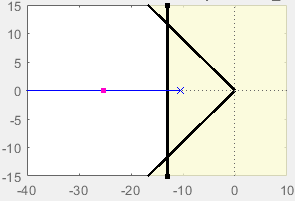
\includegraphics[width=0.45\textwidth]{images/rlocusnocontrol.png}
\caption{Lugar de las raíces del motor sin control}
\label{fig:rlocus1}
\end{figure}
\begin{figure}[!h]
\centering
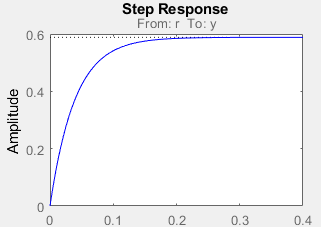
\includegraphics[width=0.45\textwidth]{images/stepnocontrol.png}
\caption{Respuesta al escalón del motor sin control}
\label{fig:step1}
\end{figure}

En La Figura\ref{fig:rlocus1} las lineas negras representan los requerimientos de tiempo y sobre-impulso, lo cual indican que se cumplen, pero en la Figura\ref{fig:step1} se aprecia que tiene un error de estado estacionario. Por ello se decide emplear un polo en s = 0 y mejora la respuesta.
Con ello se logra conseguir un error de cero , pero cambia el lugar de las raíces y no hay una ganancia que nos permita cumplir las otras especificaciones por lo que es necesario un cero. Así dar como resultado las Figuras\ref{fig:rlocus3} y \ref{fig:step4}, se opta por colocarlo en -10.4, justo sobre el polo más significativo y una ganancia proporcional K = 10.8. 

\begin{figure}[!h]
\centering
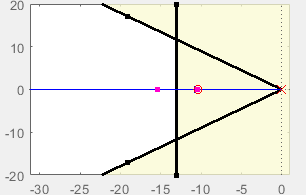
\includegraphics[width=0.45\textwidth]{images/rlocuspid.png}
\caption{Lugar de las raíces del motor con control PID}
\label{fig:rlocus3}
\end{figure}
\begin{figure}[!h]
\centering
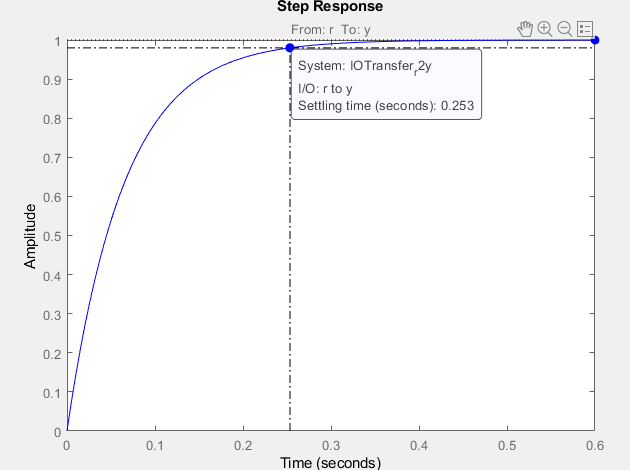
\includegraphics[width=0.45\textwidth]{images/stepfinal.png}
\caption{Respuesta al escalón del motor con control PID}
\label{fig:step4}
\end{figure}


\subsection{Obtención de parámetros $K_p$ y $K_i$}

Con la herramienta \textit{residue} de maltab se realizó la descomposición en paralelo del regulador $PI(s)$, la propuesta del regulador se convierte de la función de transferencia a la siguiente forma:

\begin{equation}
    PI(s)= \dfrac{K_c(s-z_0)}{s}= K_p + \dfrac{K_i}{s}
    \label{EQ_2}
\end{equation}

A partir de la descomposición en matlab se obtuvieron los parámetros:

\begin{equation}
    K_p=1.3598
    \label{EQ_4}
\end{equation}

\begin{equation}
    K_i=14.1422
    \label{EQ_5}
\end{equation}

De esta manera la ecuación del controlador:

\begin{equation}
    PI(s)= 1.3598 + \dfrac{14.1422}{s}
    \label{EQ_6}
\end{equation}

Ya habiendo obtenido todos los parámetros necesarios para construir el control PID, se simula los incluso con una perturbación para recrear una posible situación en el motor.

\begin{figure}[h]
\centering
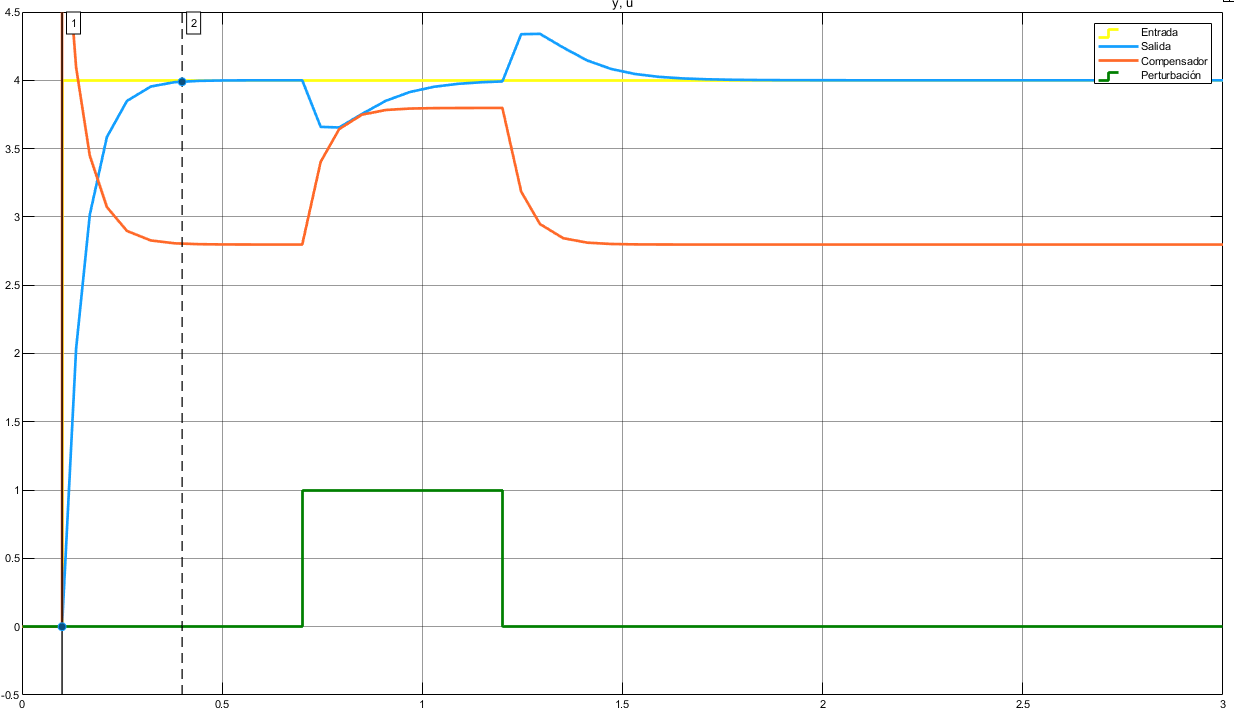
\includegraphics[width=0.5\textwidth]{images/Sumalcioncompleta.png}
\caption{Resultado de las simulación completa del motor con control}
\label{fig:RSF}
\end{figure}

\subsection{Resultados experimentales del controlador}

Mediante la herramienta LabControl se crea los componentes con los valores obtenidos de los cálculos en matlab y se introducen al motor, dando como resultado la siguiente Figura\ref{fig:R_5}
 
\begin{figure}[h]
\centering
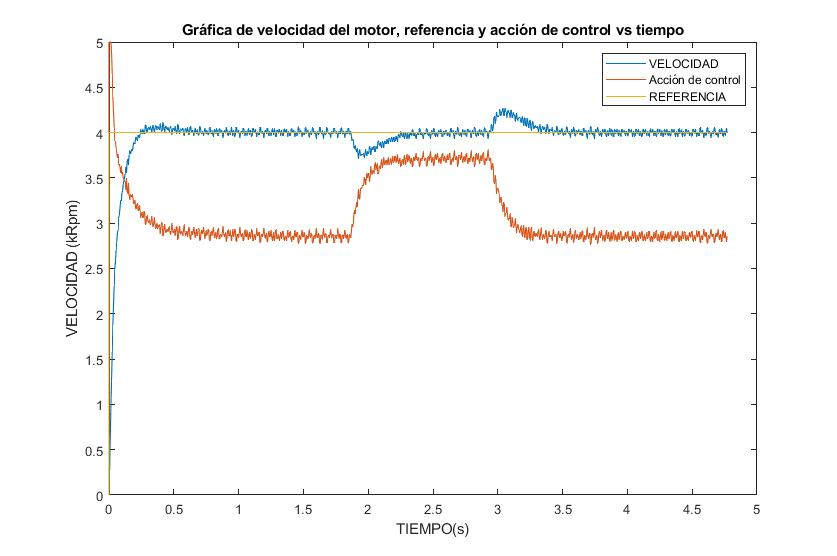
\includegraphics[width=0.5\textwidth]{images/RESULTADOS_MOTOR_CD.jpg}
\caption{Gráfica de los resultados obtenidos del motor}
\label{fig:R_5}
\end{figure}

%--------------

\begin{table}[]
    \centering
    \begin{tabular}{|c|c|}
    \hline
    $\textbf{Característica}$ & $\textbf{Valor}$ \\
    \hline
    Mp & 2.825$\%$ \\
    Ts & 205ms \\
    P & 315ms \\
    ess & 4.057 \\
    \hline
    \end{tabular}
    \caption{Resultados del experimento}
    \label{tab:tablaf}
\end{table}



\begin{figure}[!ht]
    \centering
    \begin{gnuplot}[terminal=pdf,terminaloptions={font ",20" linewidth 3},scale=0.70]
    set grid
	set ylabel 'Amplitud (V)'
	set xlabel 'Frecuencia rad/s'
	plot sin(x), cos(x), tan(x)
    \end{gnuplot}
    \caption{Relación de tensión-corriente para una bobina, utilizando una señal senoidal con una frecuencia de $f$ = 1 GHz.}
    \label{Methodolody}
\end{figure}

\section{Conclusiones}
 En la sección de conclusiones, es importante responder de manera sistemática los objetivos de la práctica dirigida partiendo desde el general hasta los específicos en prosa nunca en viñetas, para este tipo de documentos como tal. Además de los objetivos, de los resultados experimentales obtenidos y analizados previamente se debe concluir aspectos relevantes que ayuden a dar solidez del artículo o informe, por lo general es necesario ver comparaciones importante a nivel cuantitativo y no cualitativo evitando frases genéricas. Finalmente resultados no obtenidos ni discutidos en el artículo e informe no deberán aparecer en las conclusiones debido a que no tiene sentido alguno discutir de algo que no se llevó acabo.

%%%%%%%%%%%%%%%%%%%%%%%%%%%%%%%%%%%%%%%%%%%%%%%%%%%%%%%%%%%%%%%%%%%%%%%%%%%%%
% Bibliography
\bibliographystyle{IEEEtran}
\bibliography{Paper}
%%%%%%%%%%%%%%%%%%%%%%%%%%%%%%%%%%%%%%%%%%%%%%%%%%%%%%%%%%%%%%%%%%%%%%%%%%%%%
\end{document}


